The development of intelligent driver assistant systems has become a
very active research field in the last years. The large spectrum of
potential applications for such systems ranges from automatic warning
systems that detect obstacles and dynamic objects over automated
parking systems to fully autonomous cars that are able to navigate in
busy city environments. One aspect that is of major importance in all
these systems is the perception part of the vehicle, i.e., the data
acquisition and semantic interpretation of the environment. The major
challenges here include the required accuracy of the detection system,
the time constraints given by the speed of the vehicle and its implied
temporal restrictions on the decision process, as well as the large
variability in which potential objects and the environment itself may
appear. Especially this latter point poses a significant challenge on
the perception task, because standard learning techniques that most
often rely on supervised off-line classification algorithms tend to
give poor results when the test environment largely differs from the
acquired training data. Furthermore, such systems are not capable of
adapting to new, unseen situations, which reduces their applicability
for long-term use cases. 

In this paper, we present a self-supervised on-line learning algorithm
that recognizes driving behaviors and predicts appropriate actions
accordingly. A driving behavior in our context is defined as a short
sequence of actuation commands to the vehicle that typically occur in
certain traffic situations. An example is the braking maneuver in
front of a red traffic light. In our system, the driving behaviors are
observed using an inertial measurement unit (IMU) and a camera while a
human is driving the vehicle. Using our approach, the system is able
to detect and classify new traffic scenarios and predict appropriate
actions based on the driving behaviors learned in earlier stages of
the data acquisition process. The principle idea is to first segment
the data stream from the IMU into consistent sequences using
\emph{change-point detection}, and then relate these motion sequences
to visual features observed in the camera data during the
corresponding motion. To find the change-points in the motion data, we
use an efficient Bayesian approach based on a Rao-Blackwellized
particle filter. The visual features are represented in a bag-of-words
approach using a Dirichlet Compound Multinomial (DCM) model. The
detected motion segments are grouped on-line and without human
intervention, according to their similarities in their corresponding
visual features. This enables the system to predict new motion
commands according to the traffic situation it detects from new camera
data. Thus, it predicts a braking maneuver when it encounters enough
evidence for a red light in the camera data. Fig.~\ref{fig:final} shows a
typical output of our algorithm.

\begin{figure}[t]
\centering
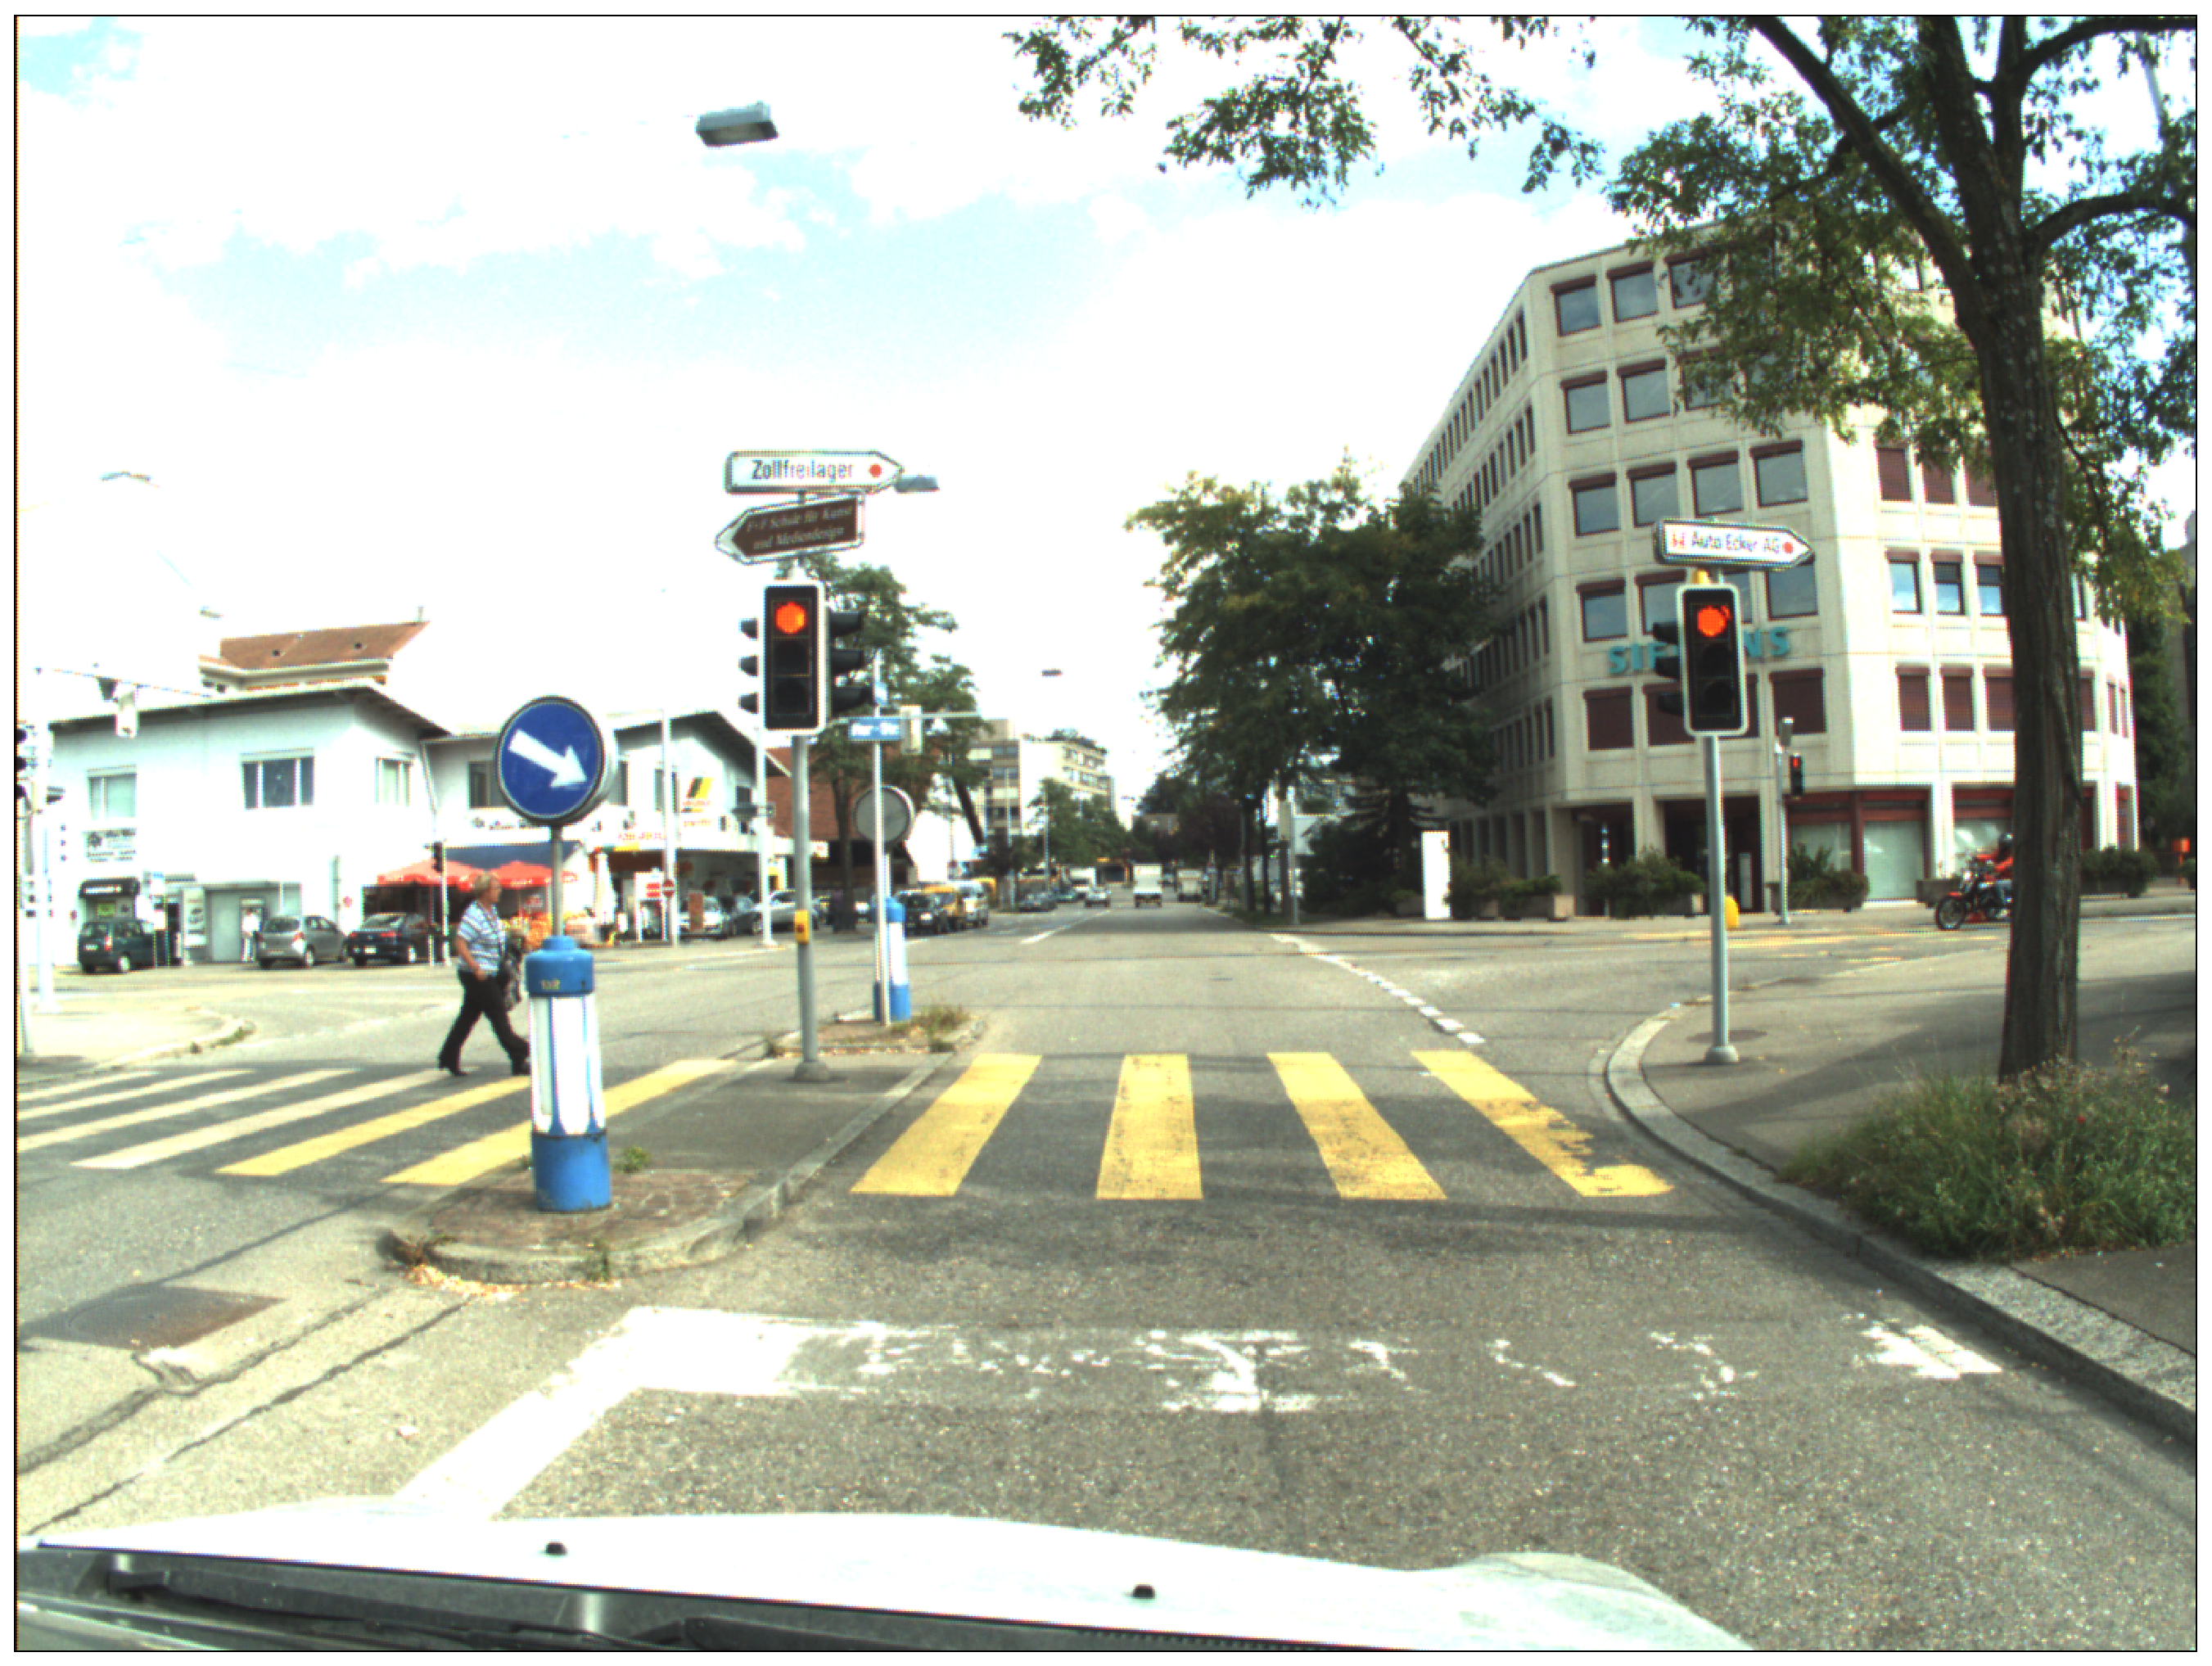
\includegraphics[width=0.65\columnwidth]{fig/place64.eps}
\caption{Driving behaviors learning and predicting in urban environments.}
\label{fig:final}
\end{figure}

The rest of the paper is structured as follows. Section~\ref{sec:related}
summarizes the previous works related to ours. Section~\ref{sec:formulation}
introduces our Bayesian framework. Section~\ref{sec:motion} describes our motion
segmentation method. Section~\ref{sec:labeling} shows how we model a traffic
situation. Section~\ref{sec:action} demonstrates our action model.
Section~\ref{sec:exp} presents experimental results. Section~\ref{sec:conc}
outlines our conclusions and provides some insights for future work.
